\documentclass[12pt]{article}
\usepackage[utf8]{inputenc}
\usepackage{amssymb}
\usepackage{amsmath}
\usepackage{textcomp}
\usepackage{graphicx}
\usepackage[a4paper, portrait, margin=1in]{geometry}
\usepackage{longtable}
\usepackage{booktabs}
\usepackage{setspace}
\usepackage[capposition=top]{floatrow}
\usepackage[style=authoryear,backend=biber,sorting=nyt,hyperref=false]{biblatex}
\addbibresource{references_10pages.bib}
\usepackage{pdflscape}
\usepackage{indentfirst}
\usepackage[implicit=false,colorlinks=true,urlcolor=blue]{hyperref}

\onehalfspacing
\begin{document}

\begin{titlepage}
	\begin{center}
		
		\vspace*{2cm}
		
		\large
		The Subprime Crisis Revisited: Unpacking the Long-Term Performance of a 2007 Bear Stearns Mortgage-Backed Securities Deal

		\vspace{1cm}		
		
		\small	
		This document contains only a few key sections of the paper. Click the link below to access the full version:
		
		\href{https://tinyurl.com/4538t3wu}{https://tinyurl.com/4538t3wu}
		
		\vspace{1cm}
		
		\large
		Alex Blumenfeld\footnote[1]{Boston University and Chicago Booth; alexblumenfeld.ab@gmail.com. Funding for this project was provided by Boston University's Undergraduate Research Opportunities Program, and by Robert King of the Boston University Department of Economics.}
		
		\vspace{0.5cm}
		
		\begin{abstract}
\noindent Residential mortgage-backed securities (RMBS) came under intense public scrutiny after the 2007 financial crisis and the subsequent Great Recession, but have since lost their status as a significant political issue. To provide some answers about whether these securities were truly as dangerous as many suspected during the crisis, I engage in a ``postmortem'' on one securitization which was issued shortly before the financial chaos of 2007: Bear Stearns Asset-Backed Securities 2006-HE10. I find that out of an original principal pool of roughly \$1.1 billion, 44.2\% of the total principal from the deal’s mortgages has been written off due to defaults, but thanks to several provisions in the deal's structure, investors have felt only 50.6\% of these losses, giving them a principal loss rate of 23.5\% through March 2020. As for the underlying mortgages, I find that foreclosures did not peak until around 2012, showing that security principal markdowns which occurred during the financial crisis itself did not capture the full extent of the mortgages’ poor performance. I also focus on two senior tranches which were purchased by the Federal Reserve’s Maiden Lane fund in 2008, when the Fed agreed to buy seemingly toxic RMBS from Bear Stearns’s portfolio to facilitate the firm’s sale to JPMorgan Chase. One of these tranches has suffered only modest principal losses, and the other has had no principal losses whatsoever, suggesting that little in-depth analysis of these securities was conducted during the height of the crisis.
		\end{abstract}
		
		\vfill
		
	\end{center}
\end{titlepage}

\section*{Introduction}
Mortgage-backed securities (MBS) burst onto the scene in the financial markets in the 1980s and 1990s, as the promise of connecting millions of mortgage borrowers with the global capital markets offered a winning outcome for everyone involved. In theory, homeowners would get lower rates on their mortgages by gaining access to capital from all over the world, investors would obtain impressive returns from a buoyant housing market by investing in a diversified portfolio of mortgages, and banks would pocket easy revenue from originating mortgages that they could immediately move off of their balance sheets. Unfortunately, a variety of forces put pressure on the incentive structure of the securitization process, and underwriting standards for non-government-guaranteed MBS began to slip by the late 1990s and early 2000s. Whereas in the past, all mortgages included in MBS loan pools were required to conform to the standards of Freddie Mac or a similar agency, this requirement was thrown out the window in the subprime market, and the quality of the underlying collateral on many deals began to drop compared to that of past securitizations. \textcite{segoviano13} describe this as one step in a “self-reinforcing credit intermediation cycle”, where a monetary incentive to securitize as many loans as possible in order to meet demand for MBS leads to weak underwriting standards, and then the complex securitization process convinces investors that these questionable loans can be combined to form a high-quality asset, boosting the demand for these attractive securities. From here, it’s not hard to imagine the markets falling further down this slippery slope: when the U.S. housing market topped out in 2007 and subsequently crashed, the formerly bulletproof mortgage-backed securities that had been flooding the market suddenly didn’t look so attractive. After the dust settled, the banks which had engaged in the opaque process of securitization, along with the credit rating agencies that assigned had AAA ratings to securitizations full of poorly performing loans, found themselves saddled with much of the blame for allowing the financial system to reach the brink of total collapse.

Now, over a decade after the credit crunch and bank bailouts of 2007 and early 2008, one means of understanding the consequences of securitization in the wake of the Great Recession is through breaking down one specific deal that fits perfectly into the trends discussed above: Bear Stearns Asset-Backed Securities (BSABS) 2006-HE10. Consisting of just over \$1B of mortgages issued just before the financial crisis, this particular deal is a great test case for exploring how securitizations performed in the wake of the Great Recession. Among other reasons, data on its historical cash flows is easily available, its performance was clearly affected by the financial crisis, and its status as a Bear Stearns-issued deal makes it relevant to the big questions economists want to ask about mortgage-backed securities’ role in the crisis. More than a decade after the Great Recession, many important questions are still lingering, such as how drastic the crisis-induced losses on MBS actually were, whether experts’ assessments of the risk level of MBS products at the height of the crisis were correct, and whether the Fed’s decision to bail out one of the nation’s largest banks was the right move. This paper cannot provide all-encompassing answers, but focusing on a single deal will at least provide the chance to get into the weeds of how mortgage-backed securities operate and react to changing economic conditions, and the process of unpacking this deal's history will hopefully provide suggestions for how similar analysis could be done in the future.

This study is most closely related to the work of \textcite{ospina18}, who assembled a much larger MBS dataset in order to ask similar questions: they concluded that losses on AAA-rated MBS in the years after the Great Recession were relatively small, and that AAA securities were in general not as aggressively mis-rated as some suspected after the crisis. The methods I use in this paper will not be able to provide similarly broad results about the performance of residential MBS as a whole, but it has the major advantage of presenting very concrete examples of how MBS issuers thought about structuring securities that could weather financial turbulence. This strategy will allow me to evaluate the more precise question of how effectively these provisions protected investors from losses, without having to aggregate across deals with conflicting structures and rules at play.

I will also focus on the two securities from this deal which played an important role in the bailout of Bear Stearns, as one of the deal's defining features is its inclusion in the Fed’s famous Maiden Lane fund. For context, in early 2008, Bear Stearns was on the verge of running out of cash, as it depended on sources of short-term funding which were close to completely drying up. In order to avoid a collapse which would cause credit markets to seize up even further, the Fed chose to facilitate the purchase of Bear’s assets by JPMorgan Chase. JPMorgan claimed that they wouldn’t be able to completely take over the remnants of Bear Stearns if they were forced to acquire the toxic MBS tranches that were still on Bear’s books, so the Fed Board of Governors authorized a \$29 billion loan to a brand-new New York Fed vehicle called Maiden Lane LLC, which would have the job of taking on the riskiest securities from what remained of Bear Stearns’s balance sheet \parencite{fcic09}. Several varieties of MBS were included, and as it turns out, two entire tranches from BSABS 2006-HE10 made their way into the Fed’s hands as part of the Maiden Lane agreement: I-A-3 (CUSIP: 07389RAC0) and II-1A-3 (CUSIP: 07389RAQ9), with initial principal balances of \$11,213,000 and \$20,339,000, respectively \parencite{fcic09}. Because these securities demonstrate the extent to which the government had to intervene in the financial system to prevent a broader collapse in 2008, it’s worth asking whether they actually caused the government to lose any money, or whether they weren’t really as toxic as JPMorgan Chase’s analysts believed during the chaos of March 2008.

In the sections that follow, I use the data from these securities' monthly investor reports to provide several perspectives on the deal’s history. Part I briefly covers background information on MBS terminology and structures, and it lays out key information about this deal’s structure. Part II provides a high-level overview of the deal’s performance and some context on important events throughout its lifetime. In Part III, I look at the deal’s mortgage pool directly, in order to learn more about the payment and delinquency patterns that would eventually result in losses for investors. Finally, in Part IV, I bring the focus back to the actual securities, by investigating to what extent investors throughout the subordination hierarchy were protected from losses on the deal’s underlying mortgages, with extra attention given to the two Maiden Lane-owned tranches. The conclusion offers further commentary on how this deal’s tumultuous life fits into the larger conversation about mortgage-backed securities and their role in the financial system.

\section*{Part I: Background and Deal Details}
\subsection*{Background}

\subsection*{Deal Details}

\section*{Part II: Timeline of Important Events and Summary of Securities' Performance}

\subsection*{Timeline}


\subsection*{Overall Levels of Writedowns}


\subsection*{Importance of ``Lower Senior'' Tranches}



\section*{Part III: The Mortgages}
\subsection*{Summary of Cash Flows}

I will now work towards a bottom-up understanding of the deal's performance since 2007 by examining its mortgage pool in greater detail. From this point onward, even though this deal’s securities are technically based on two separate groups of mortgages, Group I and Group II, the two groups will be referred to jointly when discussing their performance. Table \ref{tab:table_deal_summary} contains some useful information about the mortgages’ performance.

\begin{table}[h]
	\centering
	\caption{Mortgage Performance Summary}
	\begin{tabular}{| l  | l  |}
\hline
Mortgage pool size in January 2007 & \$1.143 billion \\
Mortgage pool size in March 2020 & \$183 million \\
Total prepayments on mortgages & \$294 million \\
Total principal remitted to the MBS trust & \$461 million \\
Total realized losses on the mortgage pool & \$510 million \\
Mortgage loss rate (realized losses divided by original pool size) & 44.6\% \\
\hline
\end{tabular}
	
	\label{tab:table_deal_summary}
\end{table}

Even just this high-level information is enough to tell a story about these mortgages’ performance: realized losses on this group of mortgages, which covered wide ranges of borrower creditworthiness, principal size, and geographic location, were over 40\% of the initial principal balance, a figure that would cause any sensible investor to shudder. This alone makes it clear that the quality of these mortgages was shaky at best. Cumulative realized losses have also exceeded the total principal payments distributed to investors since January 2007, leading to the remarkable conclusion that of all the mortgage principal that has dropped out of the deal since its inception, roughly half has been “bad” rather than “good”.

\begin{figure}[h]
	\centering
	\caption{Cross-Section of Loan Delinquency Statuses in Each Month}
	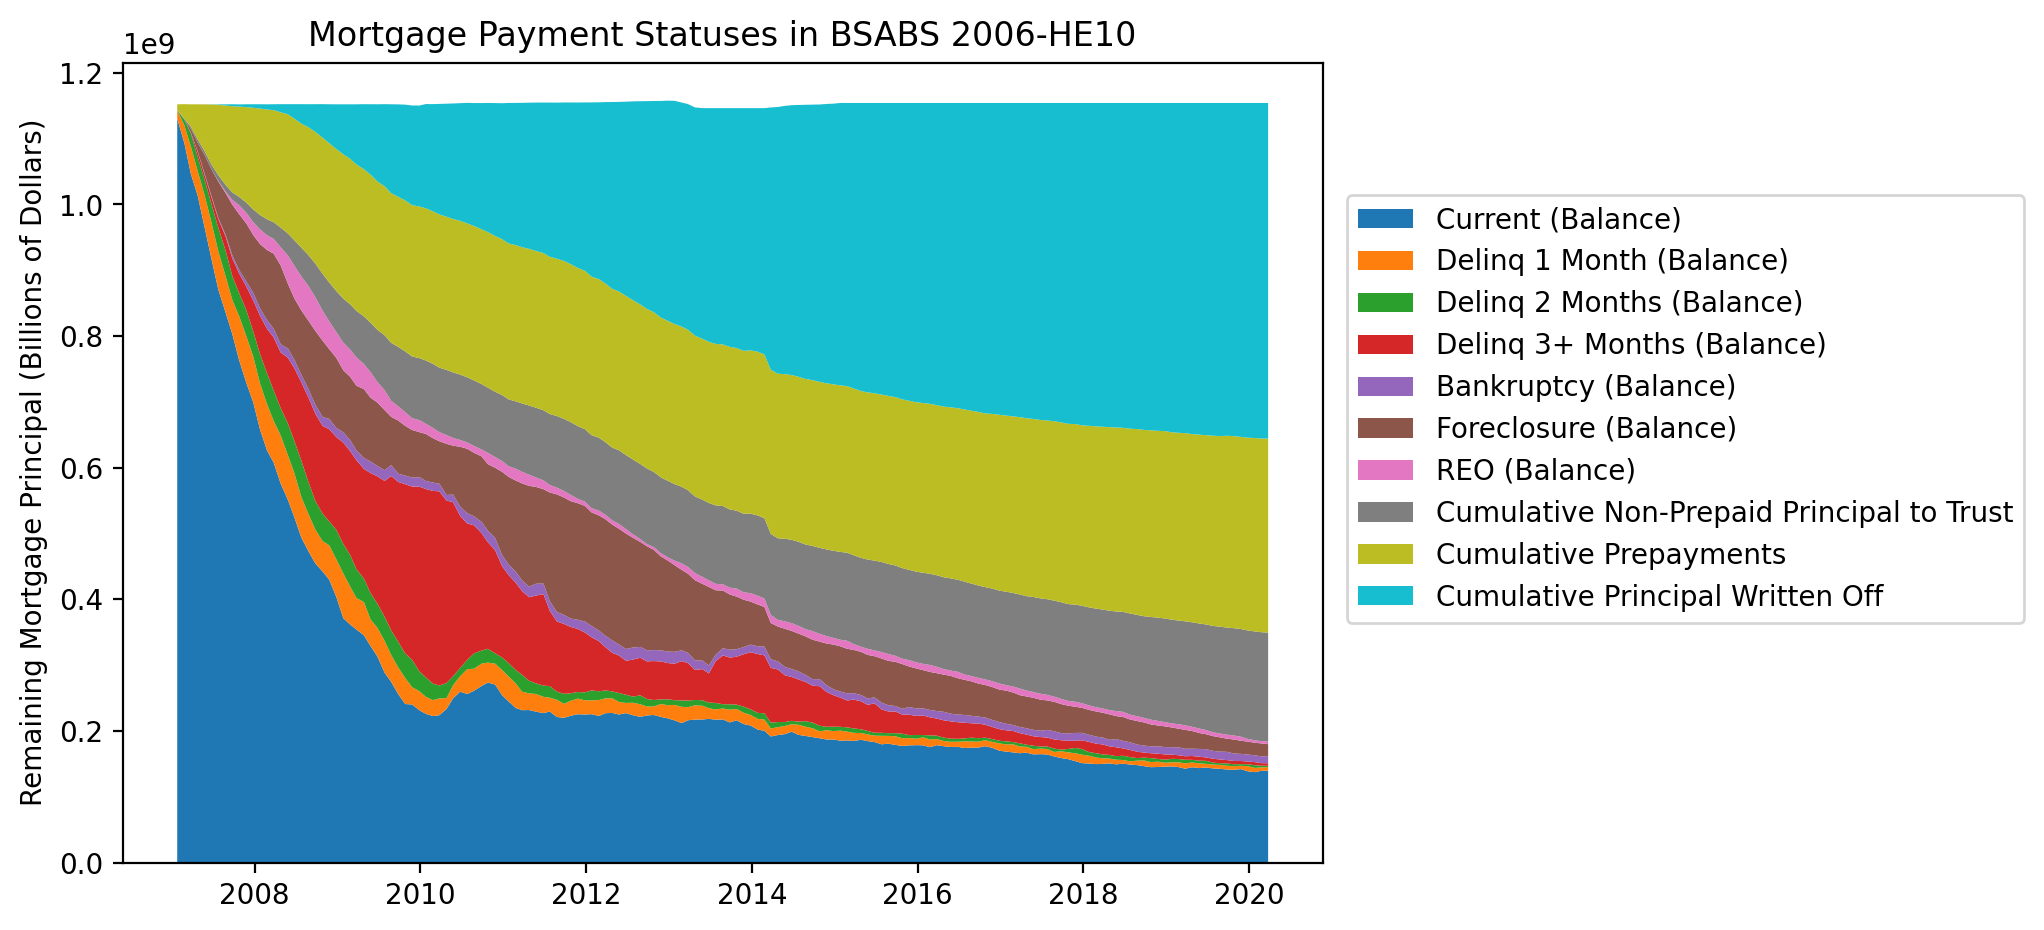
\includegraphics[width=0.8\textwidth]{../figures/stackplot_delinq_status_with_writeoffs}
	\label{fig:stackplot_delinq_status_with_writeoffs}
		\floatfoot*{Notes: This figure shows the distribution of loan statuses for all mortgages included in the deal, ranging from Current to Foreclosure/REO. It also includes the destination of every dollar of principal that has eliminated from the deal, through either payments to investors or writedowns. The number of loans in foreclosure jumped up after the Great Recession and remained relatively high until 2014. In addition, of all principal that has ``exited'' the deal, more has been written off due to mortgage defaults than has been paid out to investors.}
\end{figure}

Figure \ref{fig:stackplot_delinq_status_with_writeoffs} shows that the turmoil in housing markets in the wake of the Great Recession had effects on this deal until roughly 2014, far beyond the end of the financial crisis. Specifically, as the Great Recession reached its peak, there was a major uptick in the total value of loans for which borrowers were at least 3 months delinquent, and it took until around mid-2010 for this to fall back down. Of course, delinquency is only the beginning of the story: after the loans that are severely delinquent move through the bankruptcy process, they end up in foreclosure, where Bear Stearns would try to recoup as much of its losses as possible by selling off the borrower’s house. Once the underlying home is foreclosed on, investors become exposed to the demand for foreclosed-upon homes, not just the financials of the original borrowers. Looking at only the total loan balances held by delinquent borrowers would suggest that the detrimental effects of the Great Recession had mostly worn off by 2011 or so, but also looking at foreclosure and bankruptcy rates gives a more complete picture of how the housing market crash affected this deal. As shown by the brown region of Figure \ref{fig:stackplot_delinq_status_with_writeoffs}, it took until 2014 for the glut of foreclosed-upon loans in the deal to mostly dissipate.

	As the total remaining mortgage principal balance shrinks, the rest has to go somewhere, and that principal can be sorted in two buckets: “remittances to trust” – including prepayments and regularly scheduled payments – and “written off”. Investors receive the former, and the latter is defaulted-on principal that cannot be recovered. These two components are included at the top of Figure \ref{fig:stackplot_delinq_status_with_writeoffs}. The “Cumulative Non-Prepaid Principal to Trust” segment is calculated as total principal remitted to the trust minus total mortgage prepayments, the “Cumulative Prepayments” segment is the total value of prepayments by borrowers, and the “Cumulative Principal Written Off” segment is the sum of all realized losses on the mortgage pool over time. For an investor, it would be quite disconcerting to see that over \$500 million of the original principal balance in the mortgage pool has been written off due to defaults (as of March 2020), while slightly less than that has actually been paid out to security holders after 12 full years of mortgage payments. Part IV will provide more detail on how investors were affected by these losses.

\subsection*{Understanding the Deal's Prepayment Patterns}


\subsection*{Fixed vs. Adjustable-Rate Loans}


\section*{Part IV: Consequences for MBS Investors}

\subsection*{Where Are the Securities' Principal Payments Coming From?}

The fundamental appeal of an MBS, or any similar type of asset-backed security, is that the security’s complex structure softens the blow felt by investors when the underlying asset performs worse than expected, so the big question at hand is how much benefit that complex structure provided. This is partially about determining what fraction of losses on mortgages ended up affecting the overall group of security holders, but it’s also important to know how holders of different tranches were affected. The starting point for this analysis is Figure \ref{fig:timeseries_losses_vs_writedowns}.

\begin{figure}[h]
	\centering
	\caption{Principal Writedowns on Mortgage Pool and Securities}
	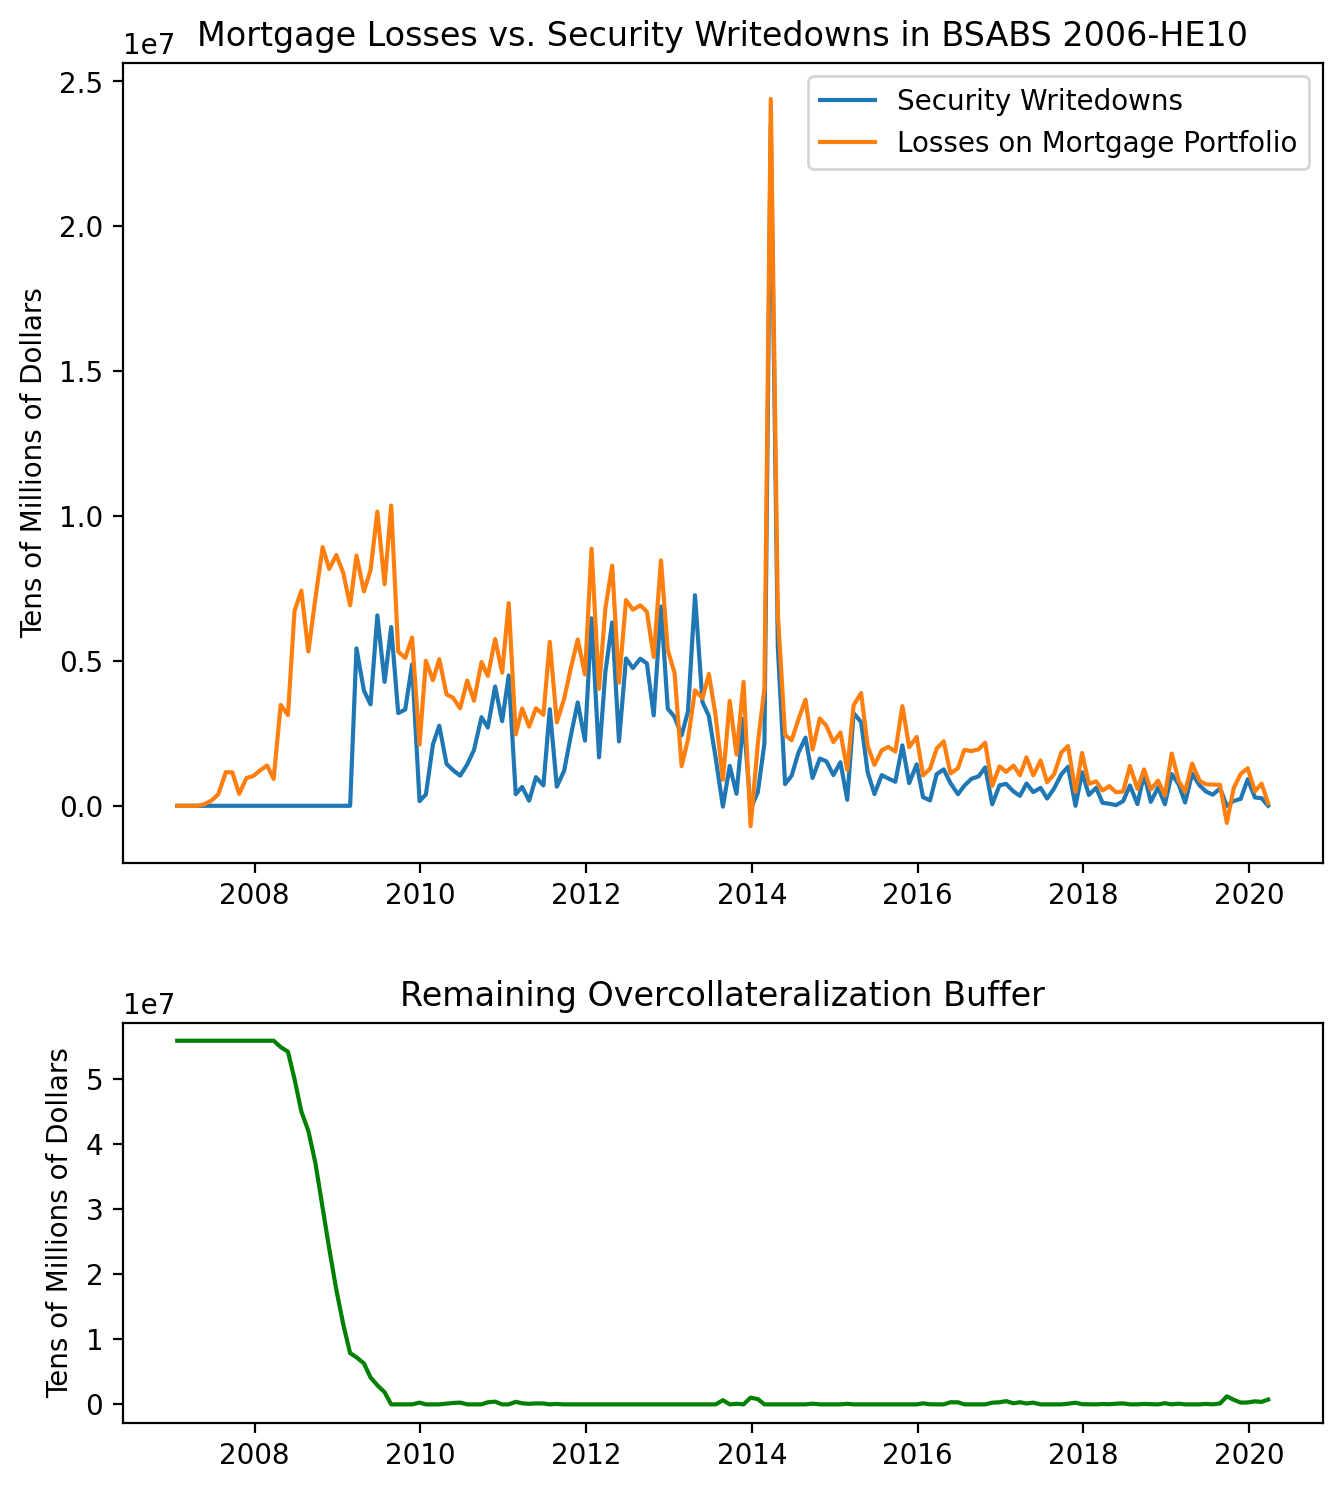
\includegraphics[width=0.8\textwidth]{../figures/timeseries_losses_vs_writedowns}
	\label{fig:timeseries_losses_vs_writedowns}
	\floatfoot*{Notes: This figure compares total principal markdowns on the securities (blue) to total defaults in the mortgage portfolio (orange). Even after the deal's overcollateralization buffer ran out, there continued to be a wedge between mortgage losses and security losses, due to the presence of excess spread coming from fixed-rate mortgages.}
\end{figure}

At a very high level, this is par for the course for a poorly performing MBS deal: the overcollateralization buffer is rapidly used up in an effort to cover mortgage losses, and writedowns on the MBS’s constituent tranches rise immediately afterwards. Perhaps surprisingly, after the initial OC buffer goes to zero, there’s still a significant gap between mortgage losses from defaulting borrowers and principal losses on securities that directly affect investors. The most likely explanations for this are excess spread due to consistent interest payments and extra cash generated by the deal’s swap agreement, so the next step is to figure out which effect dominated.

	Because the prospectus and other documents for BSABS 2006-HE10 are incredibly long and dense, it turns out that even a simple-sounding task such as trying to figure out which income streams compose the principal payments that are sent to security holders each month can be quite difficult. The data in the investor reports ultimately showed that the main sources of the cash that was sent out to investors as principal payments were 1) principal payments from the mortgages themselves, 2) interest payments from the mortgages exceeding those which had to be made to the securities, i.e. excess spread, and 3) cash coming in from the swap provider, which was negative on net. Although it’s not a perfect fit, the sum of these three components still matches up well with the series of certificate principal payments, as shown in Figure \ref{fig:timeseries_security_principal_pmts_composition}, confirming that these are the main factors at play.

\begin{figure}[h]
	\centering
	\caption{Main Components of Principal Payments Received by Securities}
	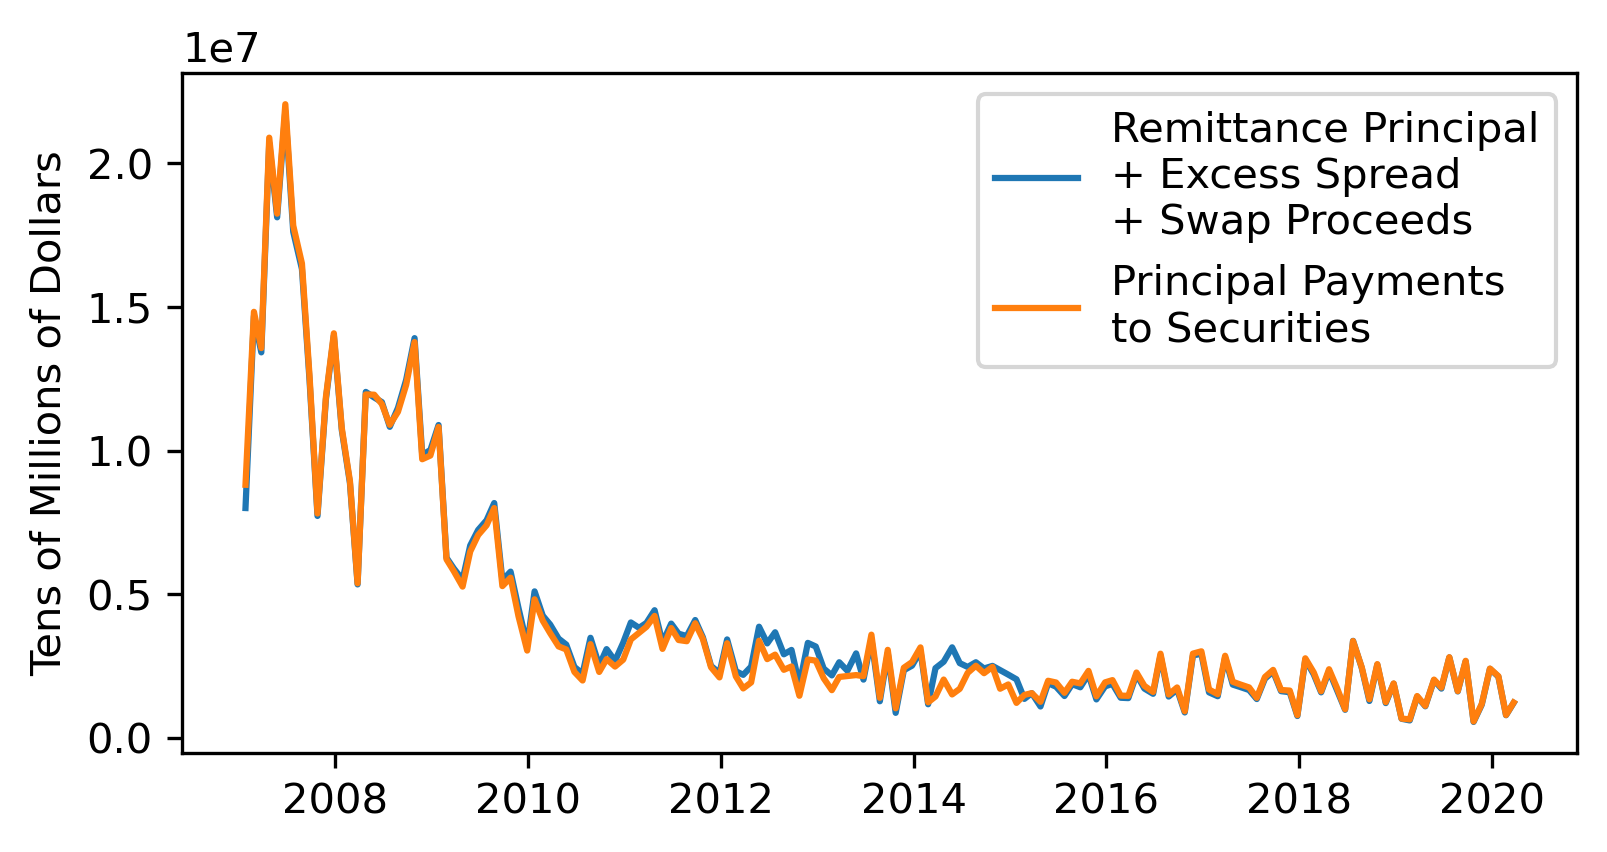
\includegraphics[width=0.7\textwidth]{../figures/timeseries_security_principal_pmts_composition}
	\label{fig:timeseries_security_principal_pmts_composition}
	\floatfoot*{Notes: This figure compares the total principal payments made to the securities to the sum of three components: principal paid by mortgage borrowers, excess spread generated by borrowers' interest payments, and the net payment to the MBS trust from the swap agreement counterparty. The sum of these three cash flows mostly matches up with the total principal paid out to investors.}
\end{figure}

To calculate the true extent of excess spread created throughout this deal’s life, I need both 1) the total interest remitted from the mortgage servicer to the trust and 2) the total interest paid out to the securities each month. It turns out that from January 2007 to March 2020, the mortgages in this deal generated \$249 million of excess spread. As described in Part I, when mortgage writedowns rise, the trustee is forced to either write down an MBS tranche or use excess spread (if any is present) to pay off some security's principal. If there had been no excess spread, then in the event that the servicer had to write off some mortgage principal due to defaults, the trustee would have had no choice but to write down the lowest-rated security remaining in the deal by the full amount of the mortgage writeoffs. However, when the trustee has some extra cash available each month due to excess spread, they can make extra principal payments to the top-rated remaining security, thus reducing the magnitude of the monthly markdowns on the bottom tranche. In this deal, the sequence of events each month appears to be as follows:

\begin{enumerate}
	\item Borrowers make their mortgage payments
	\item The resulting principal and interest are sent to the trust
	\item Interest payments are made to securities
	\item Excess spread is calculated
	\item Excess spread is distributed as principal payments to the top MBS tranche
	\item The lowest MBS tranche is written down by the necessary amount to make up the difference between mortgage pool shrinkage and security balance shrinkage
\end{enumerate}

In the long run, since some of the top-level securities’ principal was being directly paid off using any available cash from excess spread, only a fraction of the principal losses on the mortgages actually flowed through to the securities as writedowns. This is one feature of the deal’s history that was specifically made possible by a low-interest-rate environment: while all of the securities paid out a floating interest rate to investors, 24\% of the mortgages were fixed-rate, so when rates dropped significantly in response to the Great Recession, the fixed-rate borrowers ended up providing more interest than what needed to be paid out on the adjustable-rate securities. While this discussion of security vs. mortgage principal shrinkage may seem like nothing more than an accounting puzzle, the result of it is that we now have a clearer understanding of how important the deal’s excess spread provision was for mitigating realized losses, and we can see that it played a much larger role than the other available credit enhancement mechanism, the initial overcollateralization buffer.


\subsection*{The Swap Agreement}

\subsection*{To What Extent Were Investors Protected From Mortgage Defaults?}

By summing up the three payment types described in Figure \ref{fig:timeseries_security_principal_pmts_composition} from January 2007 to March 2020, I can now reach a pivotal insight about this deal’s structure, which is that on average, every \$1 of principal received by investors in this deal corresponded to approximately \$0.69 of principal payments from mortgage borrowers, \$0.37 of excess spread from borrowers’ interest payments, and -\$0.06 being sent away to the swap provider. Since it covers the entire life of the deal, not just the time before the overcollateralization buffer was completely emptied, this highlights the importance of the excess spread mechanism for protecting investors, since a significant portion of the principal that investors received actually didn’t come from borrowers’ mortgage principal payments. The total OC buffer in this deal was roughly \$55 million at its inception in January 2007, which on its own would not have been nearly enough to meaningfully protect investors, given the very high volume of defaults throughout the Great Recession.

This “principal decomposition” fits in nicely with another important result regarding this deal’s performance, which is that from January 2007 through March 2020, only 50.6\% of the principal writeoffs on the deal’s underlying mortgages were actually felt by investors. This is calculated by dividing the total principal markdowns for the securities by the total realized losses in the mortgage pool. This still adds up to hundreds of millions of dollars in losses for investors, but there is something to be said for the fact that the structure of this MBS protected its investors from almost half of the defaults on the assets they were exposed to.
	
Of course, the overall “protection rate” of 49.4\% only works at the level of the entire deal, which makes it of limited use for investors, because it’s unlikely that anybody would own stakes in every single tranche. It’s worth remembering that in Group I, all of the mezzanine securities from I-M-3 down to I-M-9 were completely wiped out by writedowns, and Group II did even worse from that standpoint, with all nine II-M mezzanine tranches being written off. At first glance, when considering that more marketed securities were marked down to \$0 than were not, it looks like this deal was almost completely wiped out by the financial crisis, but as described in Part II, the mezzanine securities still made up only a small portion of the deal’s overall principal. Despite all of the public drama surrounding over-zealous speculation on high-yielding mezzanine tranches, they are still only a small proportion of the overall certificate balance of MBS deals like BSABS 2006-HE10 – the bulk of the principal is still held in the senior securities, which will take several more years to be paid off in full and have not suffered such dramatic losses.

The stratified nature of this deal does make it hard to give a single declaration as to whether investors ended up being protected from poor mortgage performance, but the results seem to be less dire than an outsider might expect. The “static” overcollateralization buffer built into each deal provided only brief protection against losses during the early days of the financial crisis, but the “dynamic” mechanism of excess spread turned out to be much more important. The prevailing low-interest-rate environment caused this second source of protection to become the dominant one for investors, because the deal ended up generating enough cash from fixed-rate interest payments to have some left over to mitigate security holders’ losses. 

\subsection*{Maiden Lane: What Happened to the Fed's Money?}

\section*{Conclusion}

\subsection*{MBS-Related Lawsuits Against Bear Stearns}

\subsection*{What Comes Next for Securitization?}


\end{document}
